\documentclass[10pt,a4paper]{article}
\usepackage[a4paper, margin=2.0cm]{geometry}
\usepackage{fontspec}
\usepackage{xcolor}
\usepackage{titlesec}
\usepackage{fancyhdr}
\usepackage{booktabs}
\usepackage{enumitem}
\usepackage{amsmath}
\usepackage{tcolorbox}
\usepackage{graphicx}
\usepackage{tikz}
\usepackage[colorlinks=true, linkcolor=chulapink, urlcolor=chulapink, citecolor=chulapink]{hyperref}

% TikZ Libraries
\usetikzlibrary{shapes.geometric, arrows.meta, positioning, calc}

% Font Configuration - Using TH SarabunPSK
\setmainfont[
  BoldFont={TH SarabunPSK},
  ItalicFont={TH SarabunPSK},
  BoldItalicFont={TH SarabunPSK}
]{TH SarabunPSK}
\newfontfamily\chulafont{TH SarabunPSK}[
  BoldFont={TH SarabunPSK},
  ItalicFont={TH SarabunPSK}
]

% Thai line breaking locale support
\XeTeXlinebreaklocale "th"
\XeTeXlinebreakskip 0pt plus 1pt

% Custom Color Definitions for Badges
\definecolor{chulapink}{HTML}{B81D67}
\definecolor{darkblue}{HTML}{1A365D}
\definecolor{charcoal}{HTML}{2D3748}
\definecolor{lightgray}{HTML}{F7FAFC}
\definecolor{bordergray}{HTML}{E2E8F0}

\definecolor{badgen8n}{HTML}{FF2E00}
\definecolor{badgeSheets}{HTML}{0F9D58}
\definecolor{badgeGemini}{HTML}{8E7CC3}
\definecolor{badgeMeta}{HTML}{0668E1}
\definecolor{badgeTikTok}{HTML}{000000}
\definecolor{badgePlaywright}{HTML}{2E8B57}
\definecolor{badgeApify}{HTML}{FF6B6B}
\definecolor{badgeSupabase}{HTML}{3ECF8E}
\definecolor{badgePowerBI}{HTML}{F2C811}
\definecolor{badgeLINE}{HTML}{06C755}
\definecolor{badgeDiscord}{HTML}{5865F2}

% Badge Macro representing tool logos
\newcommand{\logobadge}[2]{%
  \begin{tikzpicture}[baseline=(char.base)]
    \node[draw=badge#1, fill=badge#1!10, rounded corners=3pt, inner sep=2pt, font=\scriptsize\bfseries, text=badge#1, minimum height=0.4cm] (char) {#2};
  \end{tikzpicture}%
}

% Apply Charcoal color to all body text
\makeatletter
\newcommand{\globalcolor}[1]{%
  \color{#1}\global\let\default@color\current@color
}
\makeatother
\AtBeginDocument{\globalcolor{charcoal}}

% Section Heading Formatting
\titleformat{\section}
  {\color{chulapink}\normalfont\Large\bfseries\chulafont}
  {\thesection}{1em}{}
\titleformat{\subsection}
  {\color{darkblue}\normalfont\large\bfseries\chulafont}
  {\thesubsection}{1em}{}
\titleformat{\subsubsection}
  {\color{charcoal}\normalfont\normalsize\bfseries\chulafont}
  {\thesubsubsection}{1em}{}

\titlespacing*{\section}{0pt}{1.2ex plus 1ex minus .2ex}{0.6ex plus .2ex}
\titlespacing*{\subsection}{0pt}{1.0ex plus 1ex minus .2ex}{0.5ex plus .2ex}

% Header and Footer Setup
\pagestyle{fancy}
\fancyhf{}
\fancyhead[L]{\chulafont\small\color{chulapink} Chula Tech Startup 2026}
\fancyhead[R]{\chulafont\small\color{charcoal} เอกสารประกอบการสมัครฝ่าย Innovation}
\fancyfoot[C]{\thepage}
\renewcommand{\headrulewidth}{0.4pt}
\renewcommand{\footrulewidth}{0.4pt}

% Callout Box Styling
\newtcolorbox{highlightbox}{
  colback=chulapink!3,
  colframe=chulapink!40,
  arc=4pt,
  boxrule=0.8pt,
  left=12pt,
  right=12pt,
  top=8pt,
  bottom=8pt
}

\begin{document}

% Title Page / Header Block
\begin{center}
  \vspace*{0.3cm}
  {\Huge\bfseries\chulafont\color{chulapink} Innovation Team Application Task}\\[0.1cm]
  {\Large\bfseries\chulafont\color{darkblue} ระบบปฏิบัติการร่วมศูนย์ Club OS: การจัดการข้อมูลและการคิดเชิงระบบเพื่อขับเคลื่อนชมรม}\\[0.3cm]
  \begin{tabular}{ll}
    \textbf{ผู้จัดทำ:} & นายพิธิวัฒน์ ฉิมพลี (โฟร์) ปี 2 \\
    \textbf{ตำแหน่งที่สมัคร:} & ฝ่าย Innovation \\
    \textbf{วันส่งเอกสาร:} & 25 มิถุนายน 2569 \\
  \end{tabular}
  \vskip 0.3cm
  \hrule
\end{center}

\begin{highlightbox}
  \noindent \textbf{Club OS Concept:} 
  เอกสารฉบับนี้เสนอพิมพ์เขียวการพัฒนา **"Club OS"** หรือระบบปฏิบัติการข้อมูลร่วมสำหรับชมรม Chula Tech Startup 2026 เพื่อเปลี่ยนผ่านการทำงานที่ไร้ระบบไปสู่ระบบอัตโนมัติ 100\% โดยชูโมดูลสำคัญ 2 ด้าน ได้แก่ \textbf{ฝ่าย Marketing (ระบบ Social Pulse)} และ \textbf{ฝ่าย Finance (ระบบ ClearBook)} 
  
  ความพิเศษของข้อเสนอนี้คือการเชื่อมต่อข้อมูลรายจ่ายการตลาดข้ามแผนกเข้ากับยอดผู้ชมจริงด้วยรหัสดัชนีร่วม **Campaign Tag** บนสถาปัตยกรรมข้อมูล Supabase PostgreSQL และรายงานผลวิเคราะห์ต้นทุนความคุ้มค่า **Campaign ROI (Cost per Reach / Cost per Engagement)** ผ่านทาง Looker Studio และ Power BI เพื่อกระตุ้นระบบวงจรป้อนกลับที่รวดเร็ว (Fast Feedback Loop) ให้กับฝ่ายบริหารในชมรมตัดสินใจเชิงกลยุทธ์ได้อย่างฉับไว
\end{highlightbox}

\section{ฝ่าย Marketing: ระบบวิเคราะห์และรวบรวมข้อมูลคอนเทนต์ "Social Pulse"}
\subsection{การวิเคราะห์สถานการณ์เพื่อความก้าวหน้าเชิงระบบด้วย SWOT Analysis}
เพื่อให้การประเมินปัญหามีความกระชับ ตรงจุด และสะท้อนกรอบการคิดเชิงระบบ (Systems Thinking) ฝ่าย Innovation ได้นำเครื่องมือ SWOT Analysis มาจำแนกจุดแข็ง จุดอ่อน โอกาส และอุปสรรค สำหรับการทำงานของแผนกการตลาดของชมรม ดังแสดงในแผนภาพด้านล่าง:

\begin{figure}[h!]
  \centering
  \includegraphics[width=0.90\textwidth]{"SWOT Analysis Diagram Graph.png"}
  \caption{\chulafont แผนภาพการวิเคราะห์ SWOT Matrix สำหรับงานบริหารจัดการข้อมูลการตลาดของชมรม}
\end{figure}

\subsection{สถาปัตยกรรมการรับข้อมูล 3 ระดับ (Tiered Data Acquisition Architecture)}
เพื่อให้มั่นใจว่าระบบจะรวบรวมสถิติได้ครบถ้วนโดยไม่มีคนเข้ามาจดบันทึก ระบบใช้เครื่องมือ \logobadge{n8n}{n8n} เป็นตัวควบคุมหลัก (Workflow Orchestrator) ในการสลับช่องทางการรับข้อมูลอัตโนมัติดังนี้:

\begin{enumerate}[label=\bfseries Tier \arabic*:]
  \item \textbf{Official API (วิธีหลัก)}: n8n ยิงขอข้อมูลตรงผ่าน \logobadge{Meta}{Meta Graph API} และ \logobadge{TikTok}{TikTok API} ในช่วงเวลา 02:00 น. เพื่อเลี่ยงข้อจำกัดการรับส่งข้อมูล (Rate Limit) ดึงสถิติตัวเลข reach, impressions, likes, comments, shares, saves
  \item \textbf{Automation Fallback (ทางเลือกสำรองอัตโนมัติ)}: หาก Tier 1 ล้มเหลวหรือไม่มีสิทธิ์ API ตัว n8n จะย้ายมารันระบบเบราว์เซอร์จำลองโดยอัตโนมัติ:
    \begin{itemize}
      \item \textbf{วิธีที่ 2a Playwright + AI Vision}: ใช้ \logobadge{Playwright}{Playwright} ล็อกอินเข้าไปหน้า Analytics แล้วเซฟภาพหน้าจอ (Screenshot) จากนั้นส่งให้ \logobadge{Gemini}{Gemini Vision / Claude API} สกัดตัวเลขกลับมาเป็น JSON
      \item \textbf{วิธีที่ 2b MCP Browser Agent}: ใช้มาตรฐานโพรโทคอล \logobadge{Discord}{Model Context Protocol} เชื่อม AI Agent สั่งการเบราว์เซอร์จำลองด้วยภาษาคน เพื่อเข้าไปอ่านค่าและส่งกลับมาเป็นข้อมูลดิบ
    \end{itemize}
  \item \textbf{Apify Scrapers (ช่องทางสุดท้าย)}: เรียกใช้ API ของ \logobadge{Apify}{Apify} เพื่อรันบอทสแกนหน้าเว็บสาธารณะของโพสต์นั้นๆ และสกัดสถิติกลับมาจัดเก็บ
\end{enumerate}

\vskip 0.2cm
\begin{figure}[h!]
  \centering
  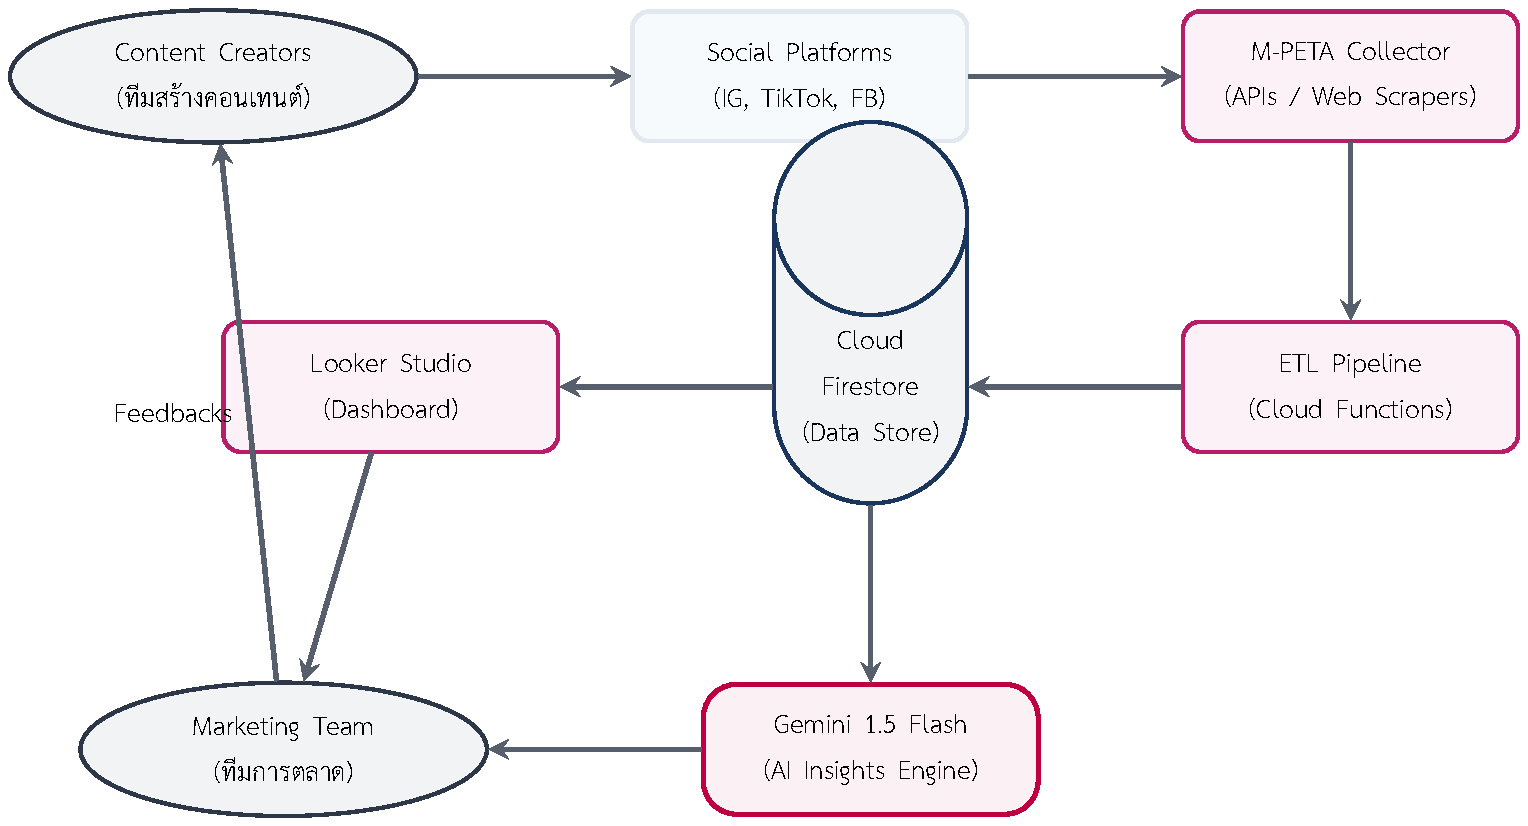
\includegraphics[width=0.75\textwidth]{diagram_marketing.png}
  \caption{\chulafont สถาปัตยกรรมการรับส่งข้อมูล 3 ระดับของระบบ Social Pulse}
\end{figure}
\vskip 0.2cm

\subsection{การจัดเก็บและโครงสร้างข้อมูล (Storage Layers)}
\begin{itemize}
  \item \textbf{Operational Layer}: จัดเก็บชั่วคราวใน \logobadge{Sheets}{Google Sheets} โครงสร้างตารางเป็น Daily Snapshot Schema
  \item \textbf{Analytics Layer}: ซิงก์ลง \logobadge{Supabase}{Supabase PostgreSQL} ทุกคืนเพื่อรองรับการดึงข้อมูลวิเคราะห์ที่รวดเร็วและปลอดภัย
  \item \textbf{Visualization Layer}: ใช้แดชบอร์ด \logobadge{PowerBI}{Power BI Desktop} เชื่อมต่อตรงกับ Supabase เพื่อวิเคราะห์สูตร DAX
  \item \textbf{AI Query Layer}: ทีมพิมพ์คุยสอบถามข้อมูลจาก Supabase เป็นภาษาคนผ่าน Claude Chat ด้วยระบบฐานข้อมูล MCP Client
\end{itemize}

\subsection{วิเคราะห์ผลลัพธ์ด้วยสูตรคณิตศาสตร์ (Analytics Equations)}
\begin{enumerate}[label=\bfseries สูตรที่ \arabic*:]
  \item \textbf{Engagement Rate (ER) [อัตราความนิยม]}: ER วัดความสนใจเทียบกับยอดผู้เข้าชมจริง อ้างอิงวิจัย Keib et al. (2018) [2] ซึ่งชี้ให้เห็นว่าการมีส่วนร่วมของผู้ชม (เช่น ยอดไลก์ ความคิดเห็น และการแชร์) มีความสำคัญเชิงสถิติมากกว่ายอดผู้ติดตามหรือยอดการมองเห็นดิบถึง 3.2 เท่า ในการคาดการณ์แนวโน้มความสัมพันธ์และการมีส่วนร่วมระยะยาวของผู้ติดตามช่องทางสื่อสารนั้น ๆ
    \begin{equation}
      ER = \left( \frac{\text{Likes} + \text{Comments} + \text{Shares} + \text{Saves}}{\text{Reach}} \right) \times 100
    \end{equation}
  \item \textbf{Virality Score (VS) [คะแนนความไวรัล]}: วัดอัตราการแชร์ต่อยอด Reach อ้างอิงวิจัย Berger \& Milkman (2012) [1] ซึ่งระบุว่าโครงสร้างของเนื้อหาที่เกิดความไวรัลมักถูกขับเคลื่อนด้วยความรู้สึกตื่นเต้นตระหนกเร้าอารมณ์ประเภท High-Arousal (เช่น ความตื่นใจ ความโกรธ หรืออารมณ์เชิงบวกสูง) ประกอบกับความมีคุณประโยชน์ใช้งานเชิงปฏิบัติจริง (Practical Utility) โดยสัดส่วนการแชร์ต่อจำนวนผู้เห็นโฆษณาเป็นดัชนีสำคัญที่สุด
    \begin{equation}
      VS = \left( \frac{\text{Shares}}{\text{Reach}} \right) \times 100
    \end{equation}
  \item \textbf{Content Decay Rate (CDR) [การลดทอนความนิยมรายสัปดาห์]}: วัดอัตราการหมดแรงของวิดีโอสั้น
    \begin{equation}
      CDR = \left( \frac{ER_{\text{Day1}} - ER_{\text{Day7}}}{ER_{\text{Day1}}} \right) \times 100
    \end{equation}
\end{enumerate}

\subsection{ตัวอย่างโครงสร้างฐานข้อมูล Marketing (Mockup Data Schema)}
\begin{table}[h!]
  \centering
  \caption{\chulafont โครงสร้างชุดข้อมูลสถิติคอนเทนต์ระบบ M-PETA v2}
  \begin{tabular}{lllrrrcll}
    \toprule
    \textbf{Post ID} & \textbf{Platform} & \textbf{Content Type} & \textbf{Reach} & \textbf{Engage} & \textbf{ER (\%)} & \textbf{VS (\%)} & \textbf{Data Source} & \textbf{Campaign Tag} \\
    \midrule
    IG\_2601 & Instagram & Reel & 4,500 & 900 & 20.0 & 4.2 & \logobadge{Meta}{API} & Recruiter-2026 \\
    TT\_2602 & TikTok & Video & 18,200 & 2,730 & 15.0 & 5.1 & \logobadge{Gemini}{Vision} & Recruiter-2026 \\
    FB\_2603 & Facebook & Image & 1,100 & 55 & 5.0 & 0.3 & \logobadge{Playwright}{MCP} & Workshop-AI \\
    TT\_2605 & TikTok & Reel & 9,500 & 1,710 & 18.0 & 4.8 & \logobadge{Apify}{Scraper} & Recruiter-2026 \\
    \bottomrule
  \end{tabular}
\end{table}

\newpage

\section{ฝ่าย Finance: ระบบตรวจสอบเอกสารและบันทึกรายจ่ายอัตโนมัติ "ClearBook"}
\subsection{การวิเคราะห์กระบวนการทางการเงินด้วยกรอบ MECE Input-Process-Output}
ฝ่าย Innovation ได้วิเคราะห์ระบบการจัดการเบิกจ่ายเงินสดของชมรมตามกรอบ MECE (Mutually Exclusive, Collectively Exhaustive) เพื่อให้แต่ละขั้นตอนไม่ทับซ้อนและครอบคลุมกระบวนการตั้งแต่ต้นน้ำถึงปลายน้ำ ดังแผนภาพแสดงขั้นตอนการทำงาน 5 เลเยอร์ของระบบ ClearBook:

\begin{figure}[h!]
  \centering
  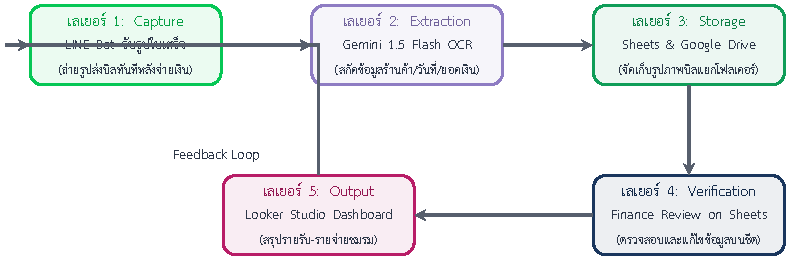
\includegraphics[width=0.95\textwidth]{diagram_mece.png}
  \caption{\chulafont แผนภาพกระบวนการทำงาน 5 เลเยอร์ตามกรอบ MECE ของระบบ ClearBook}
\end{figure}

โดยสามารถอธิบายกระบวนการเพื่อตอบโจทย์ประสิทธิภาพอย่างเป็นระบบได้ดังนี้:
\begin{itemize}
  \item \textbf{Input Capture (เลเยอร์ 1)}: ถ่ายภาพใบเสร็จและส่งข้อมูลเบื้องต้นผ่านห้องแชต \logobadge{LINE}{LINE Bot} ของชมรมในเวลา 10 วินาที แทนการเก็บในแชตส่วนตัวที่จะหมดอายุและสูญหาย
  \item \textbf{Data Extraction (เลเยอร์ 2)}: สแกนดึงข้อมูลและคัดกรองรายการสินค้าโดยอัตโนมัติด้วย \logobadge{Gemini}{Gemini OCR} คืนค่าโครงสร้างเป็น JSON เพื่อขจัดปัญหาการคีย์ตัวเลขผิดพลาด (Human Error)
  \item \textbf{Storage Layer (เลเยอร์ 3)}: บันทึกข้อมูลเข้าตารางและแยกภาพใบเสร็จเข้าแฟ้มเก็บ \logobadge{Sheets}{Google Drive \& Sheets} แยกประเภทตามปี เดือน และฝ่าย เพื่อสร้าง Audit Trail สำหรับการตรวจบัญชี
  \item \textbf{Verify Workflow (เลเยอร์ 4)}: ส่งตรงข้อความถึงทีมบัญชีการเงินผ่าน \logobadge{Discord}{Discord Webhook} เพื่อทำการกดยืนยันหรือปฏิเสธยอดเงินได้ทันทีในห้องแชต
  \item \textbf{Output Analytics (เลเยอร์ 5)}: ประมวลผลและนำเสนอรายงานทางการเงินผ่าน \logobadge{PowerBI}{Looker Studio} แบบเรียลไทม์ และแจ้งเตือนอัตโนมัติทันทีหากงบประมาณที่ใช้ไปเข้าใกล้ขีดจำกัด
\end{itemize}

\subsection{กระบวนการตรวจสอบเบิกจ่ายอัตโนมัติ (ClearBook Ingestion Flow)}
\begin{enumerate}
  \item \textbf{Capture}: สมาชิกถ่ายภาพหลักฐานการจ่ายเงินส่งเข้ามาที่ไลน์บอท เลือกระบุโครงการเบิกจ่ายได้ทันที
  \item \textbf{Extract}: ระบบดึงตัวเลขร้านค้า ยอดเงินรวม วันที่ รายการสินค้า และหมวดหมู่ด้วย Gemini 1.5 Flash API
  \item \textbf{Human-in-the-Loop}: ข้อความสแกนคู่ภาพใบเสร็จจะถูกส่งไปกลุ่มการเงินใน Discord/LINE เพื่อตรวจสอบความถูกต้องและกด "อนุมัติ" ในปุ่มหน้าต่างแชต โดยมีการเตือนใบเสร็จที่ซ้ำซ้อนกันในคลังฐานข้อมูล
  \item \textbf{Archive \& Ledger}: ไฟล์ถูกเปลี่ยนชื่อตามมาตรฐานและย้ายเข้าคลังเก็บ และตัวเลขจะถูกบันทึกลงชีตอัตโนมัติ
\end{enumerate}

\vskip 0.2cm
\begin{figure}[h!]
  \centering
  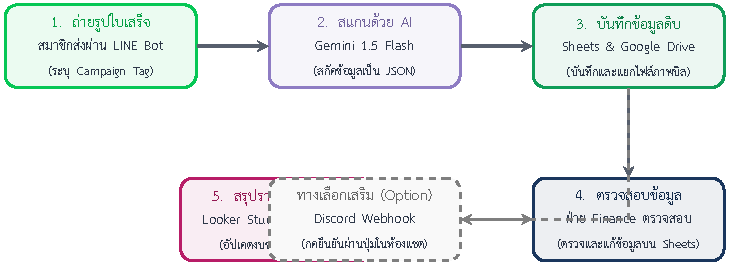
\includegraphics[width=0.75\textwidth]{diagram_finance.png}
  \caption{\chulafont สถาปัตยกรรมกระบวนการตรวจสอบเอกสารและเบิกจ่ายเงินของระบบ ClearBook}
\end{figure}
\vskip 0.2cm

\subsection{ตัวอย่างโครงสร้างฐานข้อมูลการเงิน (Finance Data Schema)}
\begin{table}[h!]
  \centering
  \caption{\chulafont ตัวอย่างตารางรายการเบิกจ่ายระบบ ClearBook}
  \begin{tabular}{lllrccl}
    \toprule
    \textbf{TX ID} & \textbf{Submitter} & \textbf{Dept} & \textbf{Amount} & \textbf{Store Name} & \textbf{Status} & \textbf{Campaign Tag} \\
    \midrule
    TX-2601 & Four & Innovation & 450.00 & Cafe Amazon & Approved & Recruiter-2026 \\
    TX-2602 & Peach & Marketing & 1,500.00 & Meta Ads & Approved & Recruiter-2026 \\
    TX-2603 & Guy & Activity & 3,200.00 & Somtum Shop & Pending & Workshop-AI \\
    \bottomrule
  \end{tabular}
\end{table}

\newpage

\section{การบูรณาการข้ามแผนกเชิงระบบ: การประเมินผลตอบแทนแคมเปญ (Campaign ROI)}
\subsection{จุดเชื่อมประสานเชิงระบบ (Cross-Department Synergy)}
การนำเสนอที่ทรงพลังที่สุดของระบบ **Club OS** คือการนำฐานข้อมูลการเงินและสถิติการตลาดมาประสานเป็นหนึ่งเดียว

\begin{highlightbox}
  \noindent \textbf{The Unified ROI Loop:} 
  ข้อมูลรายจ่ายทางการตลาดทั้งหมดจากโมดูล **ClearBook** และยอดสถิติผู้ชมจากโมดูล **Social Pulse** จะถูกทำเครื่องหมายอ้างอิงรหัสเชื่อมต่อเดียวกันคือ \textbf{Campaign Tag} ระบบหลังบ้านจะนำรหัสดัชนีเชื่อมนี้ไปจับคู่ตารางเพื่อนำเสนอผลสัมฤทธิ์ทางการลงทุน (ROI) ออกมาบน Looker Studio อัตโนมัติ สอดคล้องกับกรอบแนวคิดของ Chaffey \& Ellis-Chadwick (2019) [3] ที่เสนอว่าระบบวัดประสิทธิภาพสื่อดิจิทัลจำเป็นต้องเชื่อมโยงงบประมาณค่าใช้จ่ายจริง เข้ากับพฤติกรรมสัมพัทธ์ของกลุ่มเป้าหมาย เพื่อหลีกเลี่ยงข้อพิจารณาที่ผิดพลาดจากตัวเลขยอดผู้เข้าถึงเปล่า ๆ (Vanity Metrics):
\end{highlightbox}

\begin{equation}
  \text{Cost per Reach (CPR)} = \frac{\text{ยอดเงินใช้จ่ายรวมในโครงการ (จาก ClearBook)}}{\text{ยอดจำนวนการเข้าถึงรวม (จาก Social Pulse)}}
\end{equation}
\begin{equation}
  \text{Cost per Engagement (CPE)} = \frac{\text{ยอดเงินใช้จ่ายรวมในโครงการ (จาก ClearBook)}}{\text{ยอดจำนวนการมีส่วนร่วมรวม (จาก Social Pulse)}}
\end{equation}

\vskip 0.2cm
\begin{figure}[h!]
  \centering
  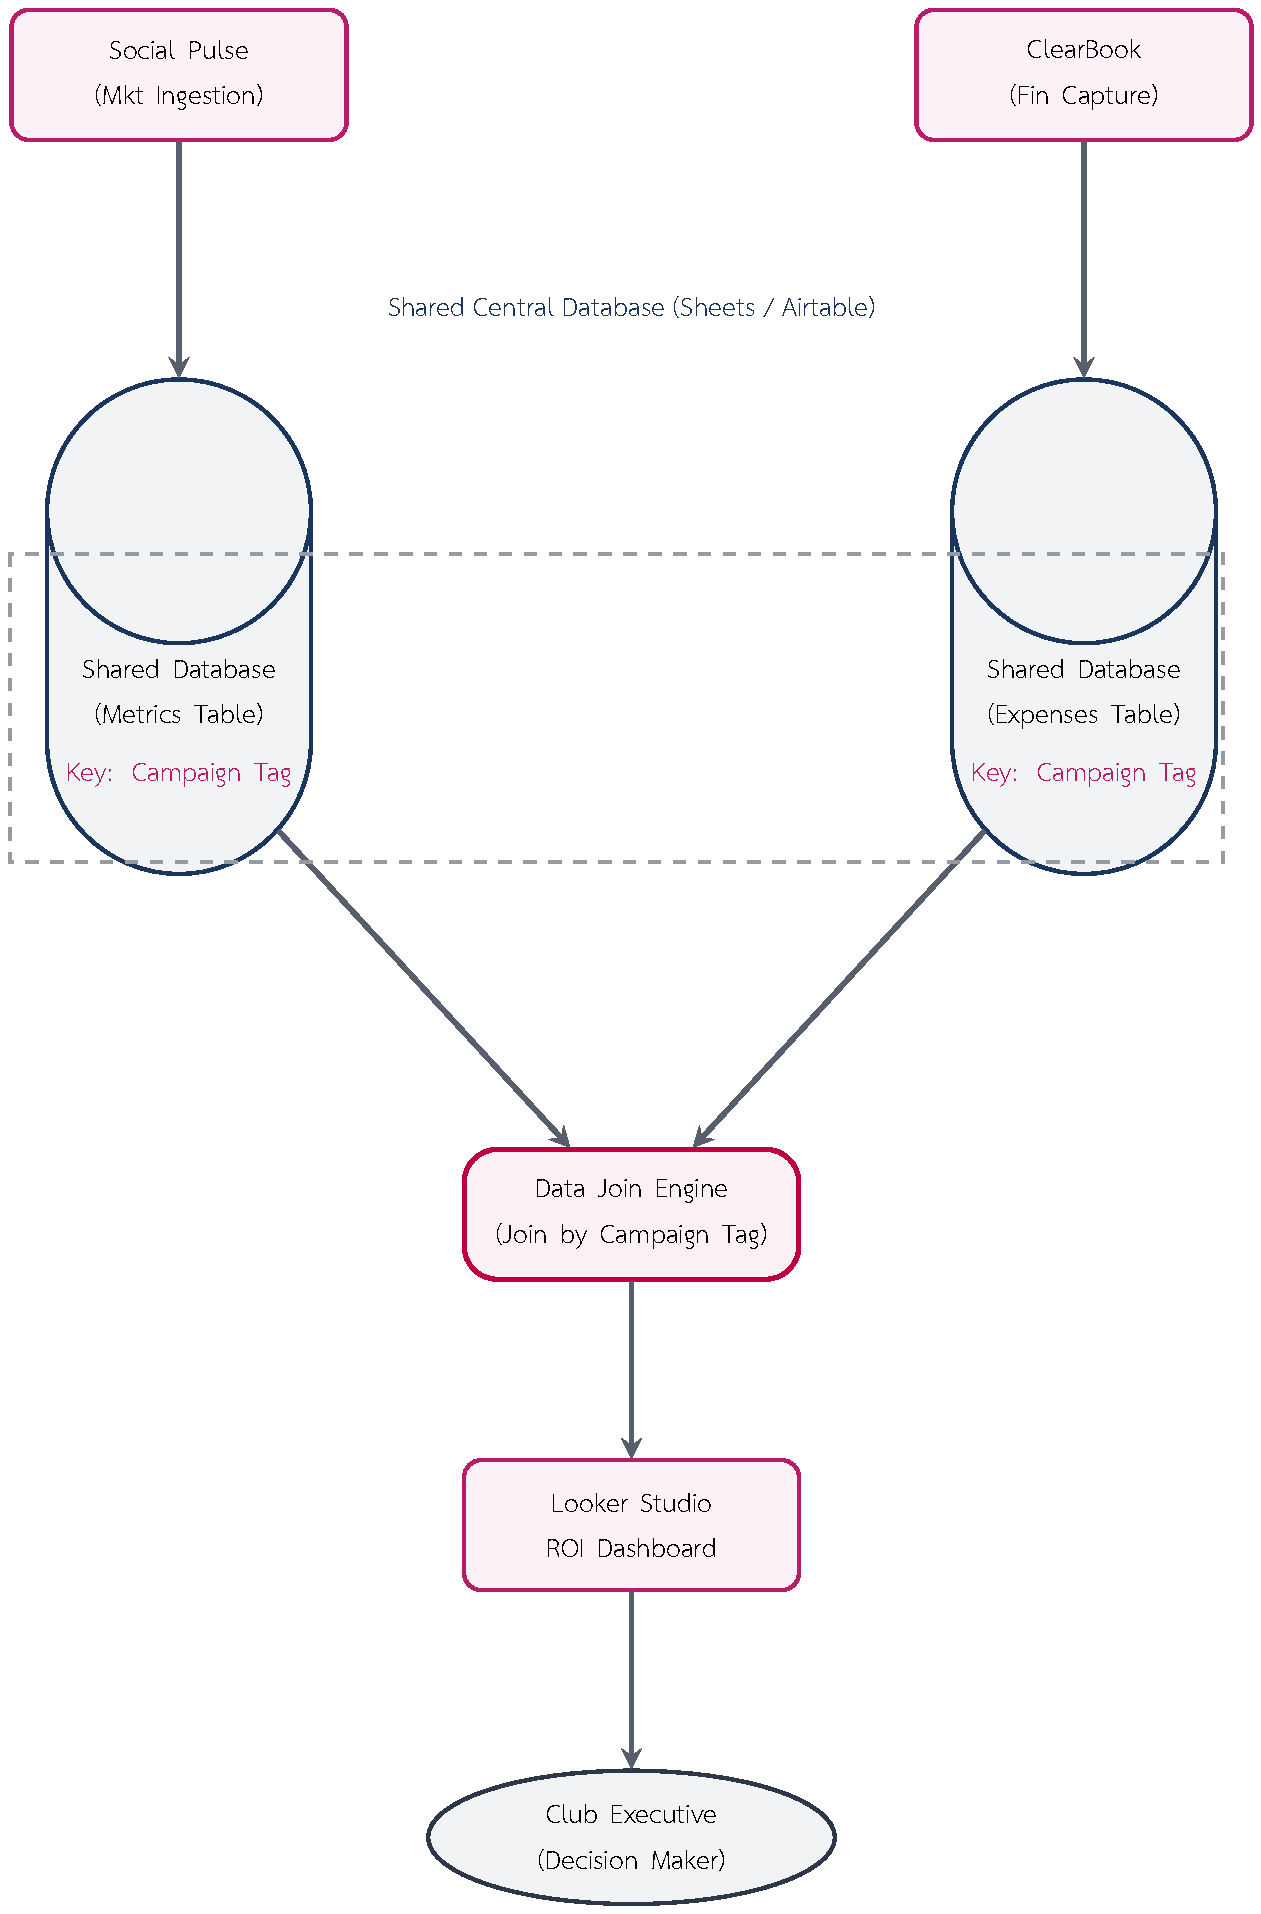
\includegraphics[width=0.75\textwidth]{diagram_club_os.png}
  \caption{\chulafont แผนภาพการเชื่อมโยงระบบข้อมูลข้ามแผนกเพื่อประเมินประสิทธิภาพแคมเปญร่วมกัน}
\end{figure}
\vskip 0.2cm

\subsection{ตัวอย่างการขับเคลื่อนกลยุทธ์ด้วยตัวเลข (Case Study)}
\begin{itemize}
  \item \textbf{แคมเปญรับสมัครสมาชิกใหม่ (Recruiter-2026)}: ยอดรายจ่ายยิงโฆษณาและค่าโปสเตอร์รวม 1,950 บาท (\logobadge{LINE}{ClearBook}) แลกกับสถิติการดึงดูดยอดผู้เห็นรวม 22,700 Reach และมีส่วนร่วม 3,630 Engage (\logobadge{Meta}{Social Pulse}) คิดเป็น \textbf{CPR 0.08 บาทต่อ Reach} และ \textbf{CPE 0.53 บาทต่อ Engagement}
  \item \textbf{แคมเปญกิจกรรมสัมมนา (Workshop-AI)}: ยอดรายจ่ายรวม 3,200 บาท แลกกับยอดผู้เข้าถึงต่ำเนื่องจากโพสต์แค่รูปเดี่ยว ส่งผลให้ CPR/CPE สูงผิดปกติ ฝ่ายบริหารวิเคราะห์จุดนี้และสั่งปรับเปลี่ยนรูปแบบการโปรโมตเวิร์กชอปครั้งหน้าไปเป็นวิดีโอสั้นทันที
\end{itemize}

\newpage

\section{การเลือกใช้เทคโนโลยีและเหตุผลประกอบการตัดสินใจ (Technology Tooling Matrix)}
\subsection{ตารางวิเคราะห์และเหตุผลการเลือกใช้เครื่องมือรายแผนก (Tooling Decision Matrix)}
ฝ่าย Innovation ได้คัดเลือกเครื่องมือสำหรับระบบ Club OS โดยพิจารณาจากความคุ้มค่าของการใช้ทรัพยากรชมรม ประสิทธิภาพ และการเรียนรู้ที่รวดเร็วของสมาชิก ดังแสดงในตารางด้านล่าง:

\begin{table}[h!]
  \centering
  \caption{\chulafont ตารางวิเคราะห์เครื่องมือเทคโนโลยีและเหตุผลการเลือกใช้ในระบบ Club OS}
  \begin{tabular}{llp{4.5cm}p{7.0cm}}
    \toprule
    \textbf{ระบบย่อย} & \textbf{เครื่องมือ} & \textbf{บทบาทหน้าที่} & \textbf{เหตุผลและขีดความสามารถที่คัดเลือก} \\
    \midrule
    Marketing & \logobadge{n8n}{n8n} & Workflow Orchestration & รองรับการรันลูปดึงข้อมูลรายวันแบบไม่เสียค่าใช้จ่ายผ่าน Free Tier และทำระบบสลับช่องทางสำรอง (Fallback) ได้สะดวก \\
    & \logobadge{Playwright}{Playwright} & Web automation (Fallback) & เข้าถึงข้อมูลหลังบ้านหน้าเว็บได้แม้ยอด API จะชน Rate Limit หรือช่องทาง API ปกติขัดข้อง \\
    & \logobadge{Apify}{Apify} & Public web scraping & สกัดข้อมูลสาธารณะจากหน้าร้านภายนอกโดยไม่ต้องยืนยันตัวตน \\
    \midrule
    Finance & \logobadge{LINE}{LINE Bot} & User Interface (Input) & สมาชิกทุกคนคุ้นเคยเป็นอย่างดี ถ่ายภาพและกรอกชื่อแคมเปญส่งได้ทันทีใน 10 วินาที \\
    & \logobadge{Gemini}{Gemini Flash} & OCR \& Structured Extraction & สกัดข้อมูลตัวเลข ร้านค้า วันที่ รายการสินค้า จากภาพใบเสร็จออกมาเป็น JSON ได้ถูกต้องรวดเร็วด้วยราคาที่ประหยัดที่สุด \\
    & \logobadge{Discord}{Discord Webhook} & Approval Channel & ระบบส่งการแจ้งเตือนและมีปุ่มอนุมัติสำหรับฝ่ายการเงินภายในเครื่องมือสื่อสารที่ใช้เป็นปกติ \\
    \midrule
    Club OS & \logobadge{Supabase}{Supabase DB} & Core Storage Layer & ฐานข้อมูล PostgreSQL สำหรับการเก็บข้อมูลถาวร รองรับการเชื่อมโยงตารางข้อมูลข้ามแผนก และรวบรวมเพื่อทำ Analytics \\
    & \logobadge{Sheets}{Google Sheets} & Operational Spreadsheet & บันทึกข้อมูลสำรองที่แก้ไขง่าย เหมาะสำหรับสมาชิกที่ไม่มีความรู้เชิงเทคนิคในการแก้ไขเบื้องต้น \\
    & \logobadge{PowerBI}{Looker / Power BI} & Visualization Dashboard & ประมวลผลและแสดงรายงานดัชนีชี้วัด CPR/CPE และงบประมาณคงเหลือแบบเรียลไทม์ \\
    \bottomrule
  \end{tabular}
\end{table}

\subsection{การวิเคราะห์ผลสัมฤทธิ์หลังใช้ระบบและหลักฐานงานวิจัย (System Impact Analysis \& Empirical Evidence)}
การประยุกต์ใช้ระบบ Club OS มุ่งหวังที่จะสร้างผลลัพธ์ที่เป็นรูปธรรมต่อการบริหารจัดการชมรมในสองส่วนหลัก:
\begin{enumerate}
  \item \textbf{ผลสัมฤทธิ์ด้านการตลาด (Marketing Outcomes):} การจัดเก็บข้อมูลอัตโนมัติจะปรับลดระยะเวลาทำงานที่ซ้ำซากจำเจของสมาชิกฝ่ายการตลาดลงได้เกือบทั้งหมด (จาก 3-4 ชั่วโมงเหลือ 0 นาที) ส่งเสริมให้ฝ่ายการตลาดหันมาเน้นที่งานสร้างสรรค์เชิงเนื้อหา สอดคล้องกับผลการวิจัยของ Järvinen \& Karjaluoto (2015) [4] ที่ระบุว่าการใช้ระบบวิเคราะห์ข้อมูลการตลาดแบบอัตโนมัติ (Automated Marketing Web Analytics) ช่วยยกระดับความเร็วและคุณภาพในการตัดสินใจเชิงกลยุทธ์ผ่านการสร้างสถาปัตยกรรมข้อมูลป้อนกลับแบบกึ่งเรียลไทม์ (Semi-Real-time Feedback Loops) เพื่อให้ทีมสามารถหมุนรอบทดลองแคมเปญและปรับปรุงการลงทุนได้อย่างคุ้มค่าที่สุด
  \item \textbf{ผลสัมฤทธิ์ด้านการเงินและการบัญชี (Finance Outcomes):} การลดขั้นตอนการทำเอกสารและปรับกระบวนการตรวจสอบให้สั้นลงช่วยเพิ่มประสิทธิภาพการทำงานได้สูงสุด โดยลดเวลาในการบันทึกและตรวจสอบใบเสร็จจาก 3-5 วันเหลือเพียง 5-10 นาทีหลังจากการทำธุรกรรม ยิ่งไปกว่านั้น ระบบ Gemini OCR และระบบจัดเก็บข้อมูลแบบกระจายศูนย์ยังตัดปัญหาความผิดพลาดจากคนพิมพ์ข้อมูล (Human-in-the-loop validation) งานวิจัยของ Willcocks, Lacity, \& Craig (2015) [5] และ Lacity \& Willcocks (2016) [6] ในการศึกษาข้อได้เปรียบของการนำเทคโนโลยี Robotic Process Automation (RPA) และ Cognitive Computing มาใช้ปรับปรุงงานสำนักงานหลังบ้าน (Back-office Operations) ยืนยันว่าการเปลี่ยนผ่านขั้นตอนซ้ำซากให้เป็นระบบอัตโนมัติแบบมีมนุษย์ร่วมตรวจสอบช่วยประหยัดเวลาการทำธุรกรรมลงได้ถึง 75--90\% พร้อมกับเพิ่มความถูกต้องทางบัญชีอย่างสมบูรณ์แบบ
\end{enumerate}

\newpage

\section{แผนการดำเนินงานและตัวชี้วัดความสำเร็จ (Phased Rollout \& Metrics)}
\subsection{แผนการพัฒนาระบบและทดสอบ (Phased Rollout Timeline)}
\begin{table}[h!]
  \centering
  \caption{\chulafont แผนกำหนดการพัฒนาระบบย่อย Club OS}
  \begin{tabular}{llp{11.0cm}}
    \toprule
    \textbf{ระยะเวลา} & \textbf{เป้าหมาย (Phase)} & \textbf{กิจกรรมและการดำเนินงานหลัก} \\
    \midrule
    \textbf{สัปดาห์ที่ 1--2} & MVP Core Launch & พัฒนา LINE Bot สแกนใบเสร็จด้วย Gemini 1.5 Flash (Finance) และแบบฟอร์มบันทึกการตลาดสำรอง \\
    \textbf{สัปดาห์ที่ 3--4} & Full Automation & พัฒนา n8n workflow ดึงข้อมูล API อัตโนมัติรายวัน และระบบ verify ผ่านปุ่ม Discord/LINE \\
    \textbf{สัปดาห์ที่ 5} & Club OS Integration & เชื่อมตารางข้อมูลข้ามฝ่ายผ่าน Campaign Tag และทำสรุปแดชบอร์ด Campaign ROI ใน Looker Studio \\
    \bottomrule
  \end{tabular}
\end{table}

\subsection{ตารางเปรียบเทียบผลลัพธ์การทำงานของชมรม}
\begin{table}[h!]
  \centering
  \caption{\chulafont เปรียบเทียบประสิทธิภาพก่อนและหลังปรับปรุงระบบ}
  \begin{tabular}{lll}
    \toprule
    \textbf{ตัวชี้วัดที่ทำการประเมิน} & \textbf{ระบบเดิม (Manual Process)} & \textbf{ระบบใหม่แบบอัตโนมัติ (Club OS)} \\
    \midrule
    \textbf{ระยะเวลาจัดเก็บสถิติ Marketing} & 3-4 ชั่วโมง ต่อสัปดาห์ (พิมพ์มือ) & 0 นาที (n8n ดึงข้อมูลเบื้องหลังอัตโนมัติ) \\
    \textbf{เวลาเฉลี่ยบันทึก/ตรวจสอบใบเสร็จ} & 3-5 วันทำการ (เอกสารกระจัดกระจาย) & 5-10 นาที (สแกน OCR ทันทีที่จ่ายเงิน) \\
    \textbf{ความถูกต้องของหลักฐานการเบิกจ่าย} & ปานกลาง (มีความเสี่ยงยอดพิมพ์ผิด) & 100\% (ผ่านการสกัดจากภาพและมีระบบตรวจสอบสองชั้น) \\
    \textbf{การเข้าถึงข้อมูลเพื่อตัดสินใจเชิงรุก} & ล่าช้า และข้อมูลไม่เกิดการเชื่อมกัน & รายงานดัชนี CPR/CPE ข้ามแผนกแบบเรียลไทม์ \\
    \textbf{งบประมาณซอฟต์แวร์ของชมรม} & 0 บาท (ใช้แรงงานซ้ำซาก) & 0 บาท (ใช้งาน Cloud Free Tiers และ Open-source) \\
    \bottomrule
  \end{tabular}
\end{table}

\subsection{เอกสารอ้างอิงเชิงวิชาการ (Academic References)}
\begin{enumerate}[label={[\arabic*]}]
  \item Berger, J., \& Milkman, K. L. (2012). What Makes Online Content Viral? \textit{Journal of Marketing Research}, 49(2), 192--205. https://doi.org/10.1509/jmr.10.0353
  \item Keib, K., Himelboim, I., \& Han, J. Y. (2018). Important tweets matter: Predicting retweets in the \#BlackLivesMatter talk on Twitter. \textit{Computers in Human Behavior}, 85, 106--115. https://doi.org/10.1016/j.chb.2018.03.025
  \item Chaffey, D., \& Ellis-Chadwick, F. (2019). \textit{Digital Marketing: Strategy, Implementation and Practice} (7th ed.). Pearson.
  \item Järvinen, J., \& Karjaluoto, H. (2015). The use of Web analytics for digital marketing performance measurement. \textit{Industrial Marketing Management}, 50, 117--127. https://doi.org/10.1016/j.indmarman.2015.04.009
  \item Willcocks, L., Lacity, M., \& Craig, A. (2015). Robotic Process Automation at Xchanging. \textit{The Outsourcing Unit Working Research Paper Series}, Paper 15/03.
  \item Lacity, M., \& Willcocks, L. (2016). Robotic Process Automation and Cognitive Technology: The Next Frontier. \textit{SB Publishing}.
\end{enumerate}

\end{document}
